\documentclass[tikz]{standalone}
\usepackage{fontawesome}
% Font
\usepackage{mathpazo}
\usepackage{libertine}
\renewcommand*\sfdefault{phv}

\large

% Color
\usepackage{xcolor}
\definecolor{f1}{HTML}{F39019}
\definecolor{b1}{HTML}{DE6A10}
\definecolor{f2}{HTML}{51A7F9}
\definecolor{b2}{HTML}{0365C0}
\definecolor{f3}{HTML}{70BF41}
\definecolor{b3}{HTML}{00882B}

% tikz
\usepackage{tikz}
\tikzstyle{every node}=[font=\sffamily]
\usetikzlibrary{shapes,arrows,positioning,calc,decorations.markings,backgrounds}
\tikzstyle{c1} = [thick,draw=b1,fill=f1]
\tikzstyle{c2} = [thick,draw=b2,fill=f2]
\tikzstyle{c3} = [thick,draw=b3,fill=f3]
\tikzstyle{cg} = [thick,draw=gray!50,fill=gray!30]
\tikzstyle{rect} = [rectangle, minimum height=1cm]
\tikzstyle{roundrect} = [rect, rounded corners=.2cm]
\tikzstyle{io} = [trapezium, trapezium left angle=70, trapezium right angle=110]
\tikzstyle{arrow} = [thick,->,>=stealth]

\tikzstyle{all} = [very thick, align=center, minimum height=1.2cm, inner xsep=.2cm]
\tikzstyle{box} = [thick,draw]
\tikzstyle{data} = [cylinder, shape border rotate=90, aspect=0.25]
\tikzstyle{vis} = [rounded corners]
\tikzstyle{mydash} = [very thick, dash pattern=on 8pt off 3.5pt, draw=gray]

\begin{document}

\begin{tikzpicture}
\node (sm) [box, all] {Sensemaking \\System};
\node (data) [box, all, data, below right=.5cm of sm, xshift=1cm] {Provenance \\Data};
\node (vis) [box, all, vis, below=.5cm of sm, yshift=-2cm] {Provenance\\Visualization};
\node (user) [all, left=5cm of data, scale=2.5, yshift=0.08cm] {\LARGE{\faUser} \\[-0.27cm] \tiny{User}};

\draw [arrow, all] (sm) node[right=.2cm of sm,yshift=.25cm] {\rmt{\textbf{capture}}} -| (data);
\draw [arrow, all] (data) |- (vis) node[midway, yshift=.25cm, xshift=-1.2cm] {\rmt{\textbf{visualize}}};
\draw [<->,>=stealth, all, mydash] (sm) -- (vis) node[midway, xshift=.3cm,rotate=-90] {\rmt{\textcolor{gray}{link}}};
\draw[arrow, all, draw=gray] ($(user.north) - (0,0.5)$) |- (sm.west) node[midway, xshift=1.1cm, yshift=.25cm] {\textcolor{gray}{\rmt{use}}};
\draw[arrow, all] (vis.west) -| ($(user.south) + (0,0.5)$) node[midway, xshift=1.1cm, yshift=.25cm] {\textbf{\rmt{support}}};

\end{tikzpicture}

\end{document}